
%
\section{Combined results}
\label{sec:results}

\begin{figure}[htbp`]
  \centering
\subfigure[]{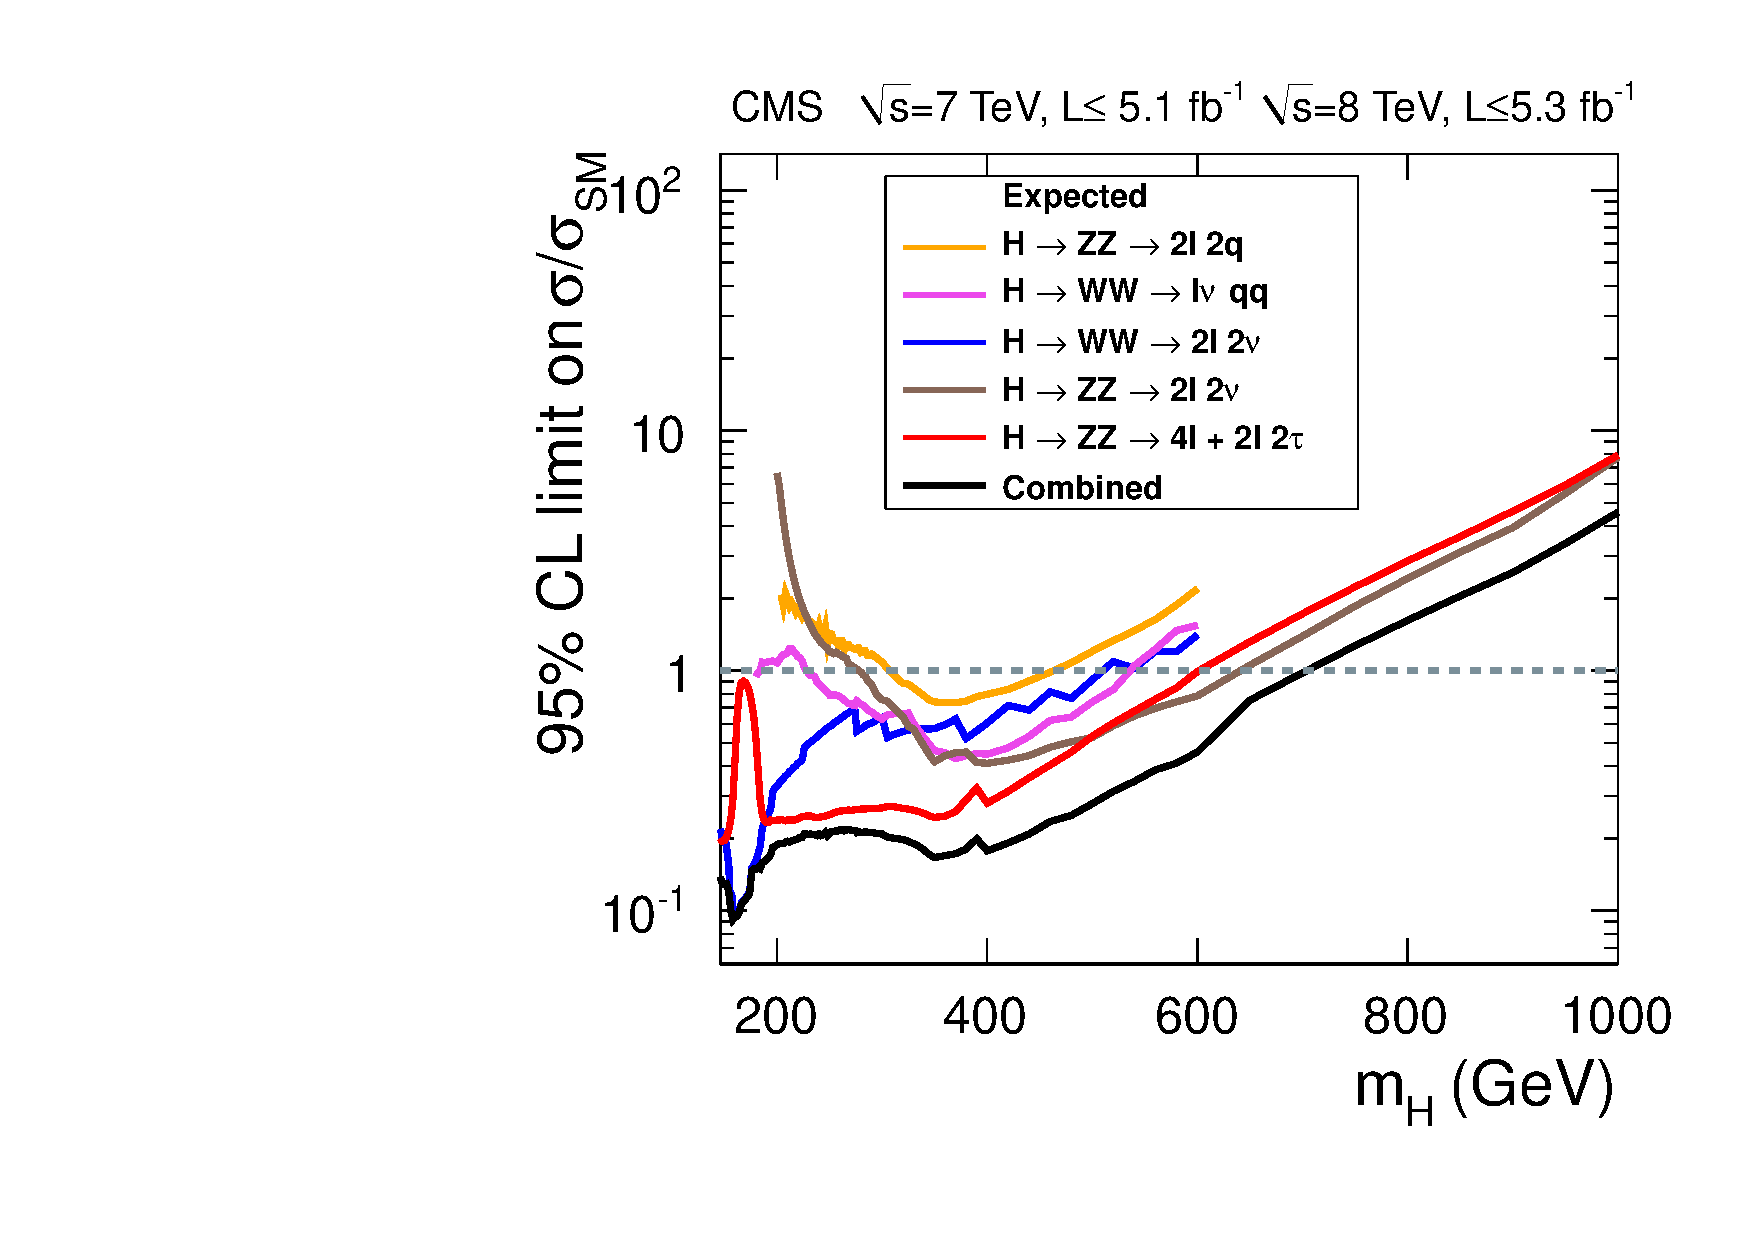
\includegraphics[width=0.45\textwidth]{figures/AllLimitsExpected.pdf}}
\subfigure[]{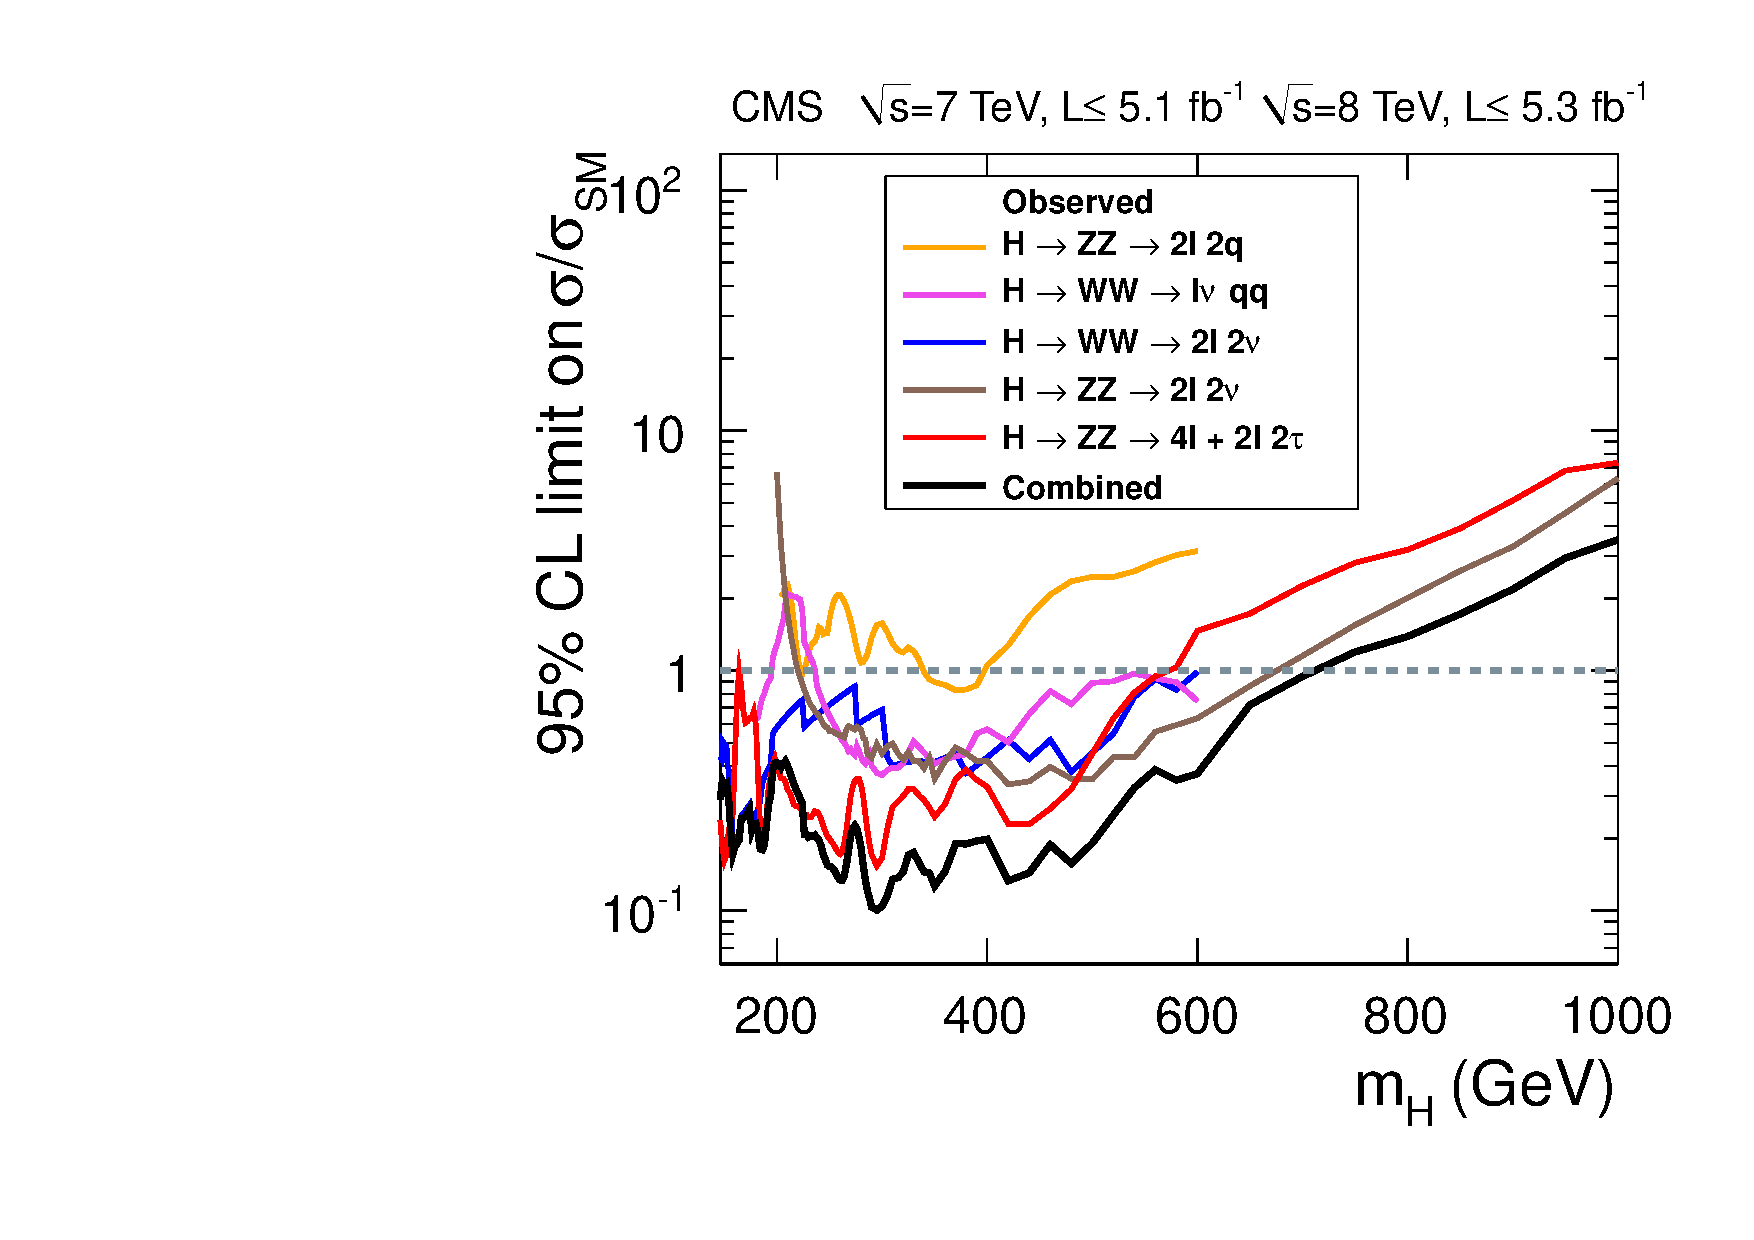
\includegraphics[width=0.45\textwidth]{figures/AllLimitsObserved.pdf}}
  \caption{\label{fig:AllLimits} (a) Expected and  (b) observed limits
  for all invividual channels compared with the combined limit.}
\end{figure}

The upper limits on the ratio of the production cross section for the Higgs boson
compared to the SM expectation for each of the individual channels presented in
this paper are plotted together in Fig.~\ref{fig:AllLimits} for (a) expected and (b)
observed limits.
Solid black lines represent the respective limits with all the channels combined
using the methods outlined in 
Refs.~\cite{LHC-HCG-Report, CMScombFeb2012}. 
The combination assumes the relative branching fractions predicted by the SM and takes 
into account the experimental statistical and
systematic uncertainties as well as the theoretical uncertainties.
The combined observed and expected limits are presented together in Fig.~\ref{fig:combined}. 
The observed values
are shown by the solid line.
The dashed  line indicates the median of the expected results for
the background-only hypothesis,
with the green (dark) and yellow (light) bands indicating the ranges in which
the CLs values are expected to lie in 68\% and 95\%
of the experiments under the background-only hypothesis.
%The probabilities for an observation, in the absence of a signal,  
%to lie above or below the 68\% (95\%) band are 16\% (2.5\%) each.
%The mass regions where the observed CLs values are below these lines are excluded
%with the corresponding (1-CLs) confidence levels.
Our previously published results exclude the SM Higgs boson from 127 to 600\GeV~\cite{Chatrchyan:2012tx}.
Results of this paper extend the upper exclusion limit to
$\mH < 710\GeV$.

\begin{figure}[htbp`]
  \centering
  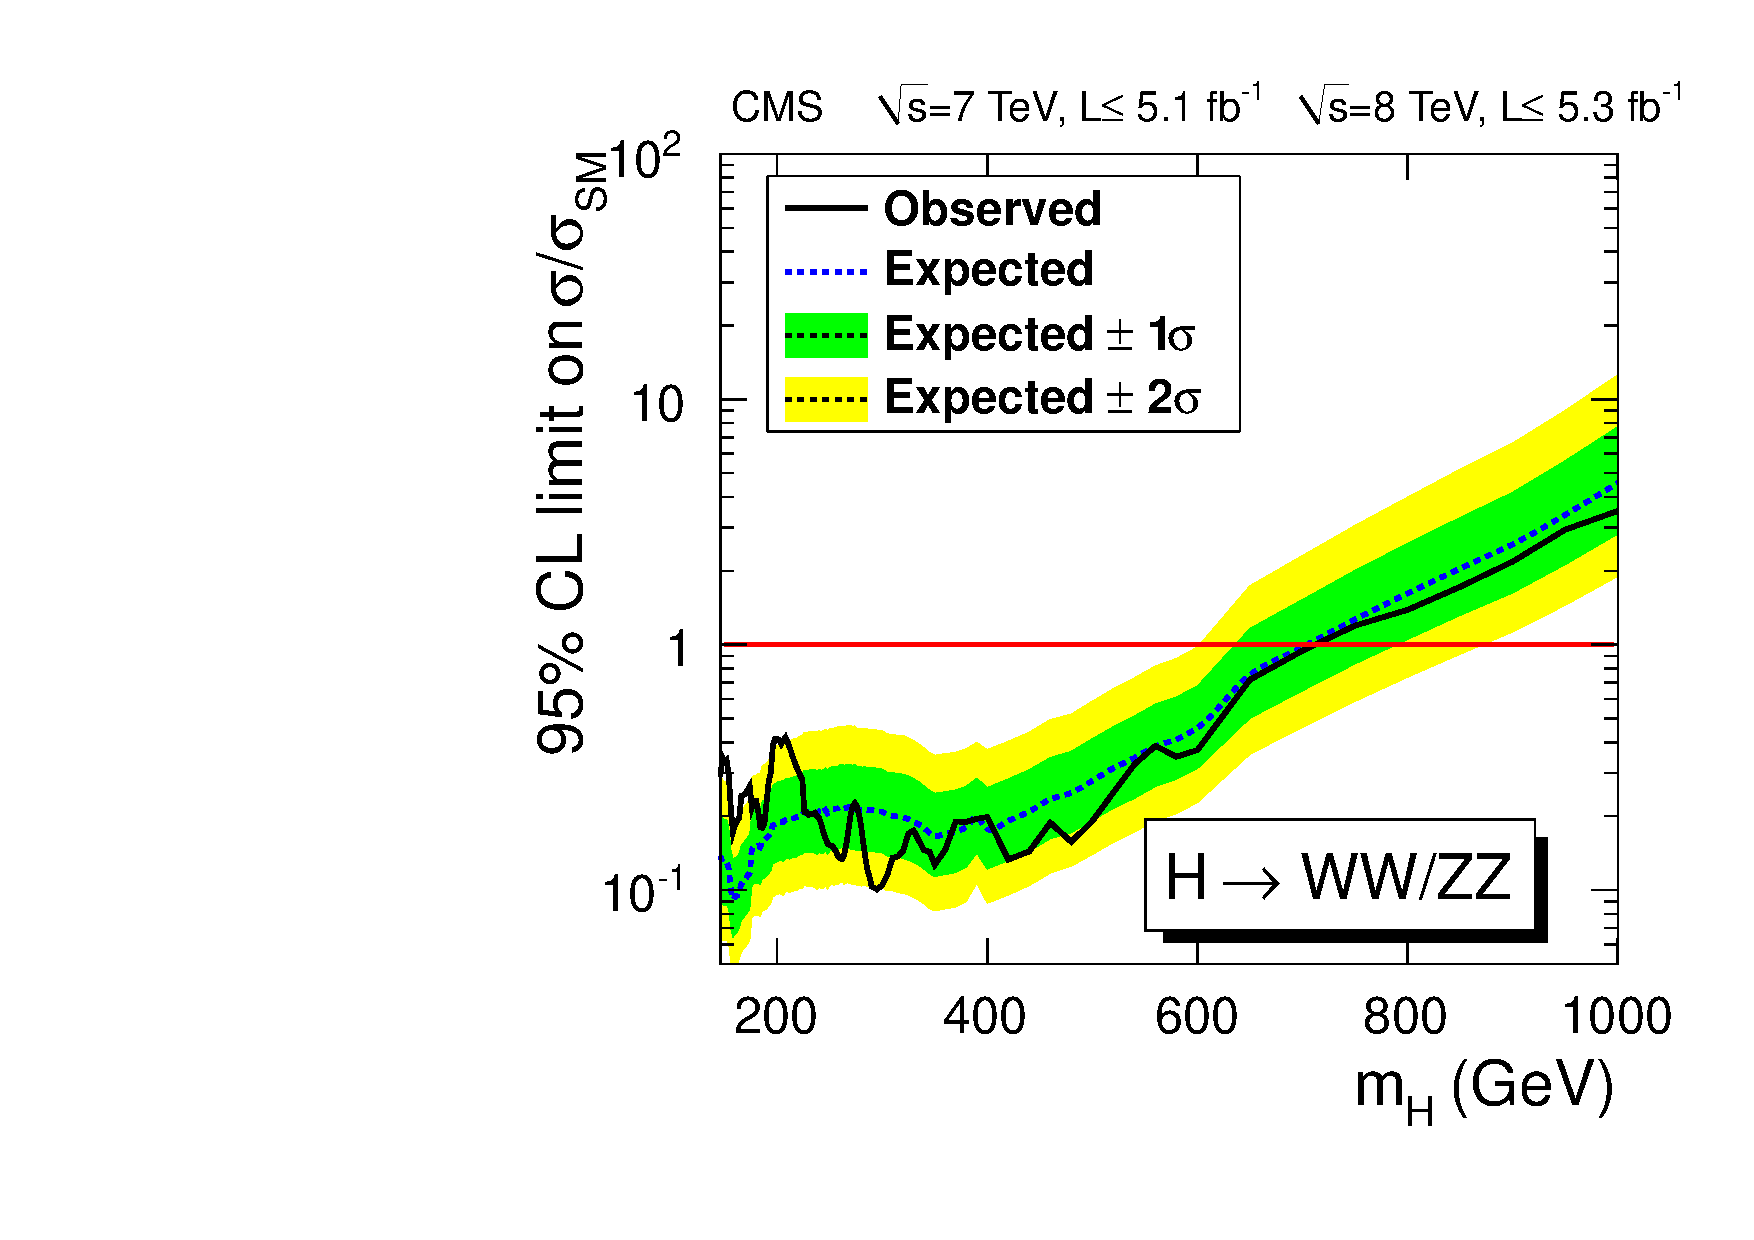
\includegraphics[width=0.6\textwidth]{figures/CombinedLimit.pdf}
  \caption{\label{fig:combined}Observed (solid) and expected
  (dashed) 95\% CL upper limit on the ratio of the production cross
  section to the SM expectation for the Higgs boson with all $\WW$ and $\ZZ$
  channels and run eras combined.}
\end{figure}


%%
\section{Summary}
\label{sec:summary}

Results are presented from searches for a standard-model-like Higgs boson in $\PH \to \WW$ 
and $\PH \to \ZZ$
decay channels  
for the Higgs-boson-mass hypotheses in the range $145 < \mH < 1000$ GeV.
The final states are studied  containing 
 two leptons and two neutrinos, $\PH \to
\WW \to \ell\nu\ell\nu$ and 
$\PH \to \ZZ \to 2\ell 2\nu$, a lepton and two jets, 
$\PH \to \WW \to \ell \nu \mathrm{qq}$,
two leptons and
two jets, $\PH \to \ZZ \to 2\ell \mathrm{q\bar{q}}$,
and four leptons, 
$\PH \to \ZZ \to 2\ell 2\ell '$, 
where $\ell = \Pe$ or $\Pgm$
and $\ell ' = \Pe$ or $\Pgm$, or $\Pgt$.
The analyses use proton-proton 
collision data recorded by the CMS detector at the LHC,
corresponding to integrated luminosities of 5.1 ${\rm fb}^{-1}$ at 
$\sqrt{s} = 7\TeV$
and 5.3 ${\rm fb}^{-1}$ at $\sqrt{s} = 8\TeV$.
The results  are found 
to be consistent with the standard model expectations with background processes only.
Upper limits at 95\% confidence level exclude a standard-model-like Higgs boson in the range  145--710 GeV,
while the expected exclusion range is 145--700 GeV.

